\documentclass[Ex4_Zusammenfassung.tex]{subfiles}

\begin{document}
\chapter{Starke Wechselwirkung und Quarkstruktur von Hadronen}
\textbf{von Anton, HeinStein, Martina \& HerMitsch}
\subsection{zur Erinnerung}
Es existieren 6 Quarks, 6 Antiquarks. Diese
\begin{itemize}
	\item können nicht alleine existieren (Confinement-Hypothese).
	\item 3 Quarks bilden ein Baryon
	\item 2 Quarks ein Meson
	\item Quarks/Antiquarks besitzen 3 mögliche Farbladungen/Antifarbladungen: $r,g,b\ \text{und } \overline{r}, \overline{g}, \overline{b}$
	\item Gluonen tragen 2 Farbladungen. Die möglichen Kombinationen sind:
		\begin{itemize}
			\item[] $r\ol{b},\ b\ol{r}$ \qquad $\frac{1}{\sqrt{2}}\lp  r\ol{r} - g\ol{g} \rp$
			\item[] $r\ol{g},\ g\ol{r}$ \qquad $\frac{1}{\sqrt{6}}\lp  r\ol{r} + g\ol{g} - 2b\ol{b} \rp$
			\item[] $b\ol{g},\ g\ol{b}$ \qquad $\frac{1}{\sqrt{3}}\lp r\ol{r} + g\ol{g} + b\ol{b}  \rp$ (wobei diese Kombination neutral ist, also sozusagen nicht zählt. )
		\end{itemize}
\end{itemize}
Gluonen \textbf{tauschen} die Farbladungen von Quarks:
\begin{figure}[h]
	\centering
	\begin{subfigure}{0.3\textwidth}
		\centering
			\feynmandiagram [horizontal=a to b] {
				i1  -- [anti fermion, edge label=$b$] a -- [anti fermion, edge label=$r$] i2 [particle=$q$],
				a -- [gluon, edge label=$r\ol{b}$, momentum'] b,
				f1 -- [anti fermion, edge label=$r$] b -- [anti fermion, edge label=$b$] f2 [particle=$q$]
			};
	\end{subfigure}
	\quad
	\begin{subfigure}{0.3\textwidth}
		\centering
		\feynmandiagram [horizontal=a to b] {
			i1  -- [anti fermion, edge label=$g$] a -- [anti fermion, edge label=$r$] i2 [particle=$q$],
			a -- [gluon, edge label=$g\ol{r}$, rmomentum'] b,
			f1 -- [anti fermion, edge label=$r$] b -- [anti fermion, edge label=$g$] f2 [particle=$q$]
		};
	\end{subfigure}
	\quad 
	\begin{subfigure}{0.3\textwidth}
		\centering
		\feynmandiagram [horizontal=a to b] {
			i1  -- [anti fermion, edge label=$b$] a -- [anti fermion, edge label=$r$] i2 [particle=$q$],
			a -- [gluon, edge label=$r\ol{b}$, momentum'] b,
			f1 -- [anti fermion, edge label=$\ol{b}$] b -- [anti fermion, edge label=$\ol{r}$] f2 [particle=$\ol{q}$]
		};
	\end{subfigure}
	\caption{Feynman-Diagramme des Farbladungsaustausches 2er Quarks (bzw. eines Quarks und Antiquarks)}
\end{figure}

\section{Mesonen}
9 Kombinationen für Mesonen. $u,s,d$--Quarks als \textbf{pseudoskalare Mesonen}:
\begin{table}[h]
	\centering
	$
	\begin{array}{cccrrc}
		\textbf{Meson} & \textbf{Quark--Kombination} & I & I_3 & S & \textbf{Masse}/\si{MeV} \\ \hline
		\pi^- & d\ol{u} & 1 & -1 & 0 & 140 \\ 
		\pi^+ & u\ol{d} & 1 & 1 & 0 & 140 \\ 
		\pi^0 & \frac{1}{\sqrt{2}} \lp d\ol{d} - u\ol{u} \rp & 1 & 0 & 0 & 135 \\ 
		K^+ & u\ol{s} & \nicefrac{1}{2} & \nicefrac{1}{2} & +1 & 494 \\ 
		K^0 & d\ol{s} & \nicefrac{1}{2} & -\nicefrac{1}{2} & +1 & 498 \\ 
		K^- & s\ol{u} & \nicefrac{1}{2} & -\nicefrac{1}{2} & -1 & 494 \\ 
		\ol{K}^0 & s\ol{d} & \nicefrac{1}{2} & \nicefrac{1}{2} & -1 & 498 \\ 
		\eta & \frac{1}{\sqrt{6}} \lp d\ol{d} + u\ol{u} + 2s\ol{s} \rp & 0 & 0 & 0 & 549 \\ 
		\eta^\prime & \frac{1}{\sqrt{3}} \lp d\ol{d} + u\ol{u} + s\ol{s} \rp & 0 & 0 & 0 & 958
	\end{array}
	$
	\caption{Pseudoskalare Mesonen}
\end{table}

Lässt man $S$ und $I_3$ eine Ebene aufspannen, bilden die Mesonen dort 9 Punkte, wobei $\pi^0,\ \eta \text{ und } \eta^\prime$ im Ursprung liegen:
\begin{figure}[h]
	\centering
	\begin{tikzpicture}
		%nodes
		\node [circle, fill, inner sep=2pt, label=above right:$\pi^0$, label=above left:$\eta^\prime$, label=below left:$\eta$] at (0,0) {};
		%lines
		\draw [-latex] (-3,0) -- (3,0) node [anchor=west] {$I_3$};
		\draw [-latex] (0,-2.5) -- (0,2.5) node [above] {$S$};
		\draw [dashed] (2.5,0) node [circle, fill, inner sep=2pt, label=above right:$\pi^+$, label=below right:$1$] {} -- (1.5,2) node [circle, fill, inner sep=2pt, label=above:$K^+$]{} -- (-1.5, 2) node [circle, fill, inner sep=2pt, label=above:$K^0$]{} -- (-2.5,0) node [circle, fill, inner sep=2pt, label=above left:$\pi^-$, label=below left:$-1$]{} -- (-1.5,-2) node [circle, fill, inner sep=2pt, label=below:$K^-$]{} -- (1.5,-2) node [circle, fill, inner sep=2pt, label=below:$\ol{K}^0$]{} -- (2.5,0) -- cycle;
		\draw [dashed] (-1.5, -2) -- (1.5,2);
		\draw [dashed] (-1.5, 2) -- (1.5, -2);
		%axis 
		\draw (-0.1,2) -- (0.1, 2) node [anchor=south west] {$1$};
		\draw (-0.1,-2) -- (0.1, -2) node [anchor=north west] {$-1$};
		\draw (1.25, 0.1) -- (1.25, -0.1) node [anchor=north] {$\nicefrac{1}{2}$};
		\draw (-1.25, 0.1) -- (-1.25, -0.1) node [anchor=north] {$-\nicefrac{1}{2}$};
	\end{tikzpicture}
\end{figure}

$u,s,d$--Quarks sind die leichtesten Quarks und erzeugen die leichtesten Mesonen. Pseudoskalare Mesonen haben $J=0$, Vektormesonen haben $J=1$. Vektormesonen bestehen aus den gleichen Quarks, haben aber gleichgerichteten Spin. Da dies einem angeregten Zustand gleichkommt und eine höhere Energie bedeutet, haben Vektormesonen eine höhere Masse.
\subsubsection*{Beispiel}
\begin{table}[h]
	\centering
	$
	\begin{array}{ccc}
	\textbf{Meson} & \textbf{Zusammensetzung} & \textbf{Masse} \\ \hline
	\text{Analog zu $\pi^+$:}\ \varrho\text{--Meson} & u\ol{d} & \SI{775}{MeV} \\ 
	\text{Analog zu $K^+$:}\ K^{++}\text{--Meson} & u\ol{s} & \SI{891}{MeV}
	\end{array} 
	$
\end{table}
Vektormesonen haben eine sehr kurze Lebensdauer und zerfallen in mehrere Skalarmesonen. \\

Anschaulich:

\quad $\varrho$--Meson: $\ket{u\ol{d}} \rightarrow M=\SI{775}{MeV}$
 
\quad $\omega$--Meson: $\frac{1}{\sqrt{2}} \lp \ket{u\ol{u}} + \ket{d\ol{d}} \rp \rightarrow M=\SI{793}{MeV}$
 
 Diese beiden Mesonen sind sehr ähnlich.
\end{document}